\chapter{FUNDAMENTOS TEÓRICOS}
\section{Introducción} % {{{
El estudio de los sistemas cuánticos cerrados, es decir, sistemas que no
interactúan con su entorno, nos ha permitido entender bastante bien muchos
fenómenos cuánticos. 
%Este tipo de sistemas suponen el límite de validez para la ecuación de 
%Schrödinger~\janote{cita}.
No obstante, una descripción más precisa 
requiere de considerar que los sistemas cuánticos reales son sistemas abiertos
que interactúan con su entorno. Para estudiar los 
sistemas cuánticos abiertos será útil revisar un formalismo distinto
al del vector de estado para describir a los estados cuánticos. 
Este formalismo es el de la matriz densidad y tiene la ventaja 
de describir de manera más apropiada a los estados mixtos. 
La interpretación de la matriz densidad como la representación de los 
estados cuánticos es utilizada en información cuántica, computación cuántica, 
sistemas abiertos y otros campos en los que la preparación del estado es 
ruidoso y puede ocurrir decoherencia \cite{fano1957description,nielsen_chuang_2011,wilde2013quantum}. Nosotros adoptaremos esta interpretación
de la matriz densidad a lo largo de este texto. 
Para la descripción de la evolución dinámica  
vamos a estudiar la teoría de los canales cuánticos, 
que es un marco teórico en el cual se considera que los estados 
cuánticos (matriz densidad) evolucionan de forma discreta.

La estructura de este capítulo es la siguiente.
En la sección \ref{sec:ensambles} revisaremos una motivación para introducir 
a la matriz densidad a partir de un ensamble de estados. 
Seguidamente, en la sección \ref{sec:density-matrices-properties},
estudiaremos las propiedades que debe cumplir una matriz 
de densidad para representar un estado cuántico
y cómo se reformulan los postulados 
de la mecánica cuántica utilizando este nuevo formalismo.
En la sección \ref{sec:qtm-channels} vamos a revisar las
condiciones para que un canal cuántico describa la evolución 
física de la matriz de densida. Por último, en la sección
\ref{sec:qtm-channels-representation}, vamos a estudiar 
la representación de superoperador y de Kraus de un canal cuántico.

% }}}
\section{Ensambles de estados cuánticos} \label{sec:ensambles} % {{{
% \esqueleto{Un copy-paste de la sección 1.1 del informe final de 
% prácticas. Voy a retocar alguna parte si fuera necesario, como ser
% más formal o agregar alguna prueba.}

Para introducir la definición de la matriz densidad presentamos la 
motivación que exponen Sakurai y Napolitano \cite{sakurai_napolitano_2017}.
Consideremos un sistema cuántico que se encuentra en alguno de los estados 
$\Pk{i}$ con probabilidad $p_i$. Esto induce naturalmente el 
ensamble de estados del sistema $\{p_i, \ket{\psi_i} \}$. 
Supongamos que realizamos 
la medición de algún observable $\Lambda$ sobre el ensamble. El 
valor esperado al medir $\Lambda$ sobre este sistema es
\begin{align}\label{eq:expVal-expanded-Lambda}
	\expval{\Lambda} &= \sum_i p_i \matrixel{\psii}{\Lambda}{\psii}
	= \sum_{i,j,k} p_i 
	\bra{\psii}\dyad{\phi_j}{\phi_j}\Lambda\dyad{\phi_k}{\phi_k}\Pk{i},
\end{align}
con $\ket{\phi_j}$ es una base ortonormal del
espacio de Hilbert del sistema. Si se reordena
\eqref{eq:expVal-expanded-Lambda} de manera apropiada
se obtiene una expresión 
que motiva claramente la definición de la matriz densidad $\rho$,
\begin{align}\label{eq:expVa-Lambda-wRho}
	\expval{\Lambda}&= \sum _{j,k}\bra{\phi_k}\qty(\sum_ip_i \dyad{\psii}{\psii} 
	)\ket{\phi_j}	\matrixel{\phi_j}{\Lambda}{\phi_k}.
\end{align}
La matriz que se encuentra entre paréntesis se define como 
la matriz densidad 
$\rho$~\cite{nielsen_chuang_2011, sakurai_napolitano_2017}
\begin{equation}\label{eq:rho_def}
	\rho \equiv \sum _i p_i\dyad{\psi_i}{\psi_i}.
\end{equation}
Notemos que un elemento de matriz de $\rho$, escrita en la base 
$\ket{\phi_j}$, es
\begin{align}
	\matrixel{\phi_k}{\rho}{\phi_j} = 
	\sum_ip_i \braket{\phi_k}{\psii}\braket{\psii}{\phi_j},
\end{align}
por lo tanto, sustituyendo en la ecuación \eqref{eq:expVa-Lambda-wRho}
se tiene que el valor promedio del observable $\Lambda$ es
\begin{align}\label{eq:Tr(rhoLambda)}
	\expval{\Lambda}=\sum _k \matrixel{\phi_k}{\rho \Lambda}{\phi_k} 
	= \Tr \qty(\rho\Lambda).
\end{align} 
%Este resultado muestra cómo a partir de la matriz densidad $\rho$ 
%se puede calcular toda la información física disponible de un sistema al 
%realizar una medición. 
Este resultado es interesante porque muestra que es posible 
calcular el valor promedio de un observable utilizando la 
matriz densidad del sistema. En virtud de este resultado
vale la pena investigar a continuación cómo evoluciona la 
matriz densidad de un sistema.
%Desde luego la matriz densidad es una herramienta con la que
%se puede formular matemáticamente la mecánica cuántica como 
%con el vector de estado.
% \cpnote{Esta frase la pondría
% al principio del capítulo y lo que sigue del párrafo lo pondría al mismo 
% nivel conceptual que la discusión anterior. }. 
% \janote{De acuerdo. En la última iteración que hice de la introducción
% tome en cuenta este comentario tuyo.}
% 
% \cpnote{En aras de la simplicidad, 
% yo formularía el ejemplo directamente con al $U$. No hay necesidad de traer el 
% Hamiltoniano acá.}
% \cpnote{El título 
% de la siguiente sección contradice la ultima frase. quizá vale la pena que revises
% este caputulo y lo leas todo a ver si hay mas problemas como de estructura. }
% 

Consideremos un sistema que se encuentra en el ensamble 
de estados inicial $\{ p_i, \ket{\psi_i(0)}\}$
y que evoluciona según algún operador unitario $U(t)$. Es decir, 
el ensamble de estados en cualquier tiempo $t>0$ está dado por 
$\{p_i, U(t)\ket{\psi_i(0)}\}$. Entonces, utilizando la definición 
\eqref{eq:rho_def} recién introducida, la matriz de
densidad $\rho(t)$ del sistema será
\begin{align} \label{eq:Rho-evolution-H}
	\rho(t) &= \sum_i p_i\dyad{\psi_i(t)}{\psi_i(t)}\nonumber\\
	&= \sum_i p_i U(t) \dyad{\psi_i(0)}{\psi_i(0)}U^{\dagger}(t)
	\nonumber\\
	&= U(t)\rho(0)U^{\dagger}(t),
\end{align}
donde $\rho(0)$ es la matriz densidad del ensamble 
de estados inicial $\{p_i, \ket{\psii(0)}\}$. Hemos probado así
que la descripción dinámica de un sistema que evoluciona 
según un operador unitario puede hacerse utilizando 
su matriz densidad. En la sección que sigue 
estudiaremos las propiedades que deben satisfacer 
las matrices de densidad en general y revisaremos cómo 
formular los postulados de la mecánica cuántica con la matriz densidad.

%
%Por ejemplo, veamos a continuación cómo 
%describir la evolución de un sistema cuántico cerrado.
%Consideremos un sistema cuyo Hamiltoniano es $H$, y es
%independiente del tiempo. Bajo estas condiciones la evolución
%del sistema está descrita por 
%$\ket{\psi (t)}=U(t)\ket{\psi(0)}$~\cite{sakurai2010modern}. 
%Sin embargo, consideremos que el sistema se encuentra inicialmente
%en un ensamble de estados $\{p_i, \ket{\psii(0)}\}$, por lo cual
%el estado final del sistema será 
%$\{p_i, \ket{\psii(t)}\}$.
%Por consiguiente, el matriz densidad final $\rho(t)$  es 
%\begin{align} \label{eq:Rho-evolution-H}
%	\rho(t) &= \sum_j p_j\dyad{\psi_j(t)}{\psi_j(t)}\nonumber\\
%	&= \sum_j p_j U(t) \dyad{\psi_j(0)}{\psi_j(0)}U^{\dagger}(t)
%	\nonumber\\
%	&= e^{-iHt}\rho(0)e^{iHt},
%\end{align}
%donde $\rho(0)$ es la matriz densidad que describe al ensamble 
%de estados inicial $\{p_i, \ket{\psii(0)}\}$.	 Aunque hemos desarrollado 
%un ejemplo para la evolución de un sistema cuyo Hamiltoniano es 
%independiente del tiempo, es sencillo de ver que en general la dinámica  
%de un sistema cerrado se describe como 
%\begin{align}\label{eq:rho-ClosedEvolution}
%\rho(0) \longrightarrow U\rho(0)U^{\dagger}.
%\end{align}
%Con esto, se ha asegurado que la dinámica de un sistema cuántico puede 
%describirse utilizando su matriz densidad. 


%Las ecuaciones \eqref{eq:Tr(rhoLambda)} y \eqref{eq:rho-ClosedEvolution}
%muestran que la matriz densidad puede utilizarse para la descripción 
%de la medición y la evolución de los estados cuánticos. 
%En la siguiente sección veremos la formulación de los postulados 
%de la mecánica cuántica utilizando la matriz densidad. 


% }}}
\section{Propiedades de la matriz densidad} % {{{
% \cpnote{Aca voy. Lo anterior ya queda listo}
\label{sec:density-matrices-properties}
% \esqueleto{Revisando esta sección en el informe de prácticas 
% veo que me gustaría ir aquí más al grano y mandar al lector 
% a las pruebas en el Chuang (para no copiar otra vez las pruebas
% aquí). Puntualizaré: (1) caracterización de la matriz densidad, (2)
% postulados de la mecánica cuántica usando la matriz densidad y
% (3) matriz densidad reducida.}


A pesar de que contamos con la definición \eqref{eq:rho_def} de 
la matriz densidad dado un ensamble de estados, será útil 
estudiar cuáles son las condiciones que una matriz debe cumplir 
para ser una matriz densidad. Luego de esto, estamos listos 
para revisar la formulación de los postulados de la mecánica cuántica
utilizando la matriz densidad. Por último, vamos a estudiar la
matriz densidad reducida, la manera para describir a los
subsistemas de sistemas compuestos con el formalismo 
de la matriz densidad.

Las propiedades que una matriz debe tener para que esta represente al 
estado físico de un sistema se establecen a 
continuación~\cite{nielsen_chuang_2011}:
\begin{thm}\label{teo:density-matrix}
Una matriz $\rho$  que actúa sobre el espacio de Hilbert de un sistema 
es la matriz densidad asociada a algún ensamble 
$\{p_i, \ket{\psi _i} \}$ si y sólo si satisface las condiciones:
\begin{enumerate}
\item $\Tr \rho = 1$.
\item $\matrixel{\psi}{\rho}{\psi} \geq 0$, $\forall\ket{\psi} \in \hi$.
\end{enumerate}	
\end{thm} 
\begin{proof} Consultar~\cite[p.~101]{nielsen_chuang_2011} \end{proof}

La condición de traza unitaria de la matriz densidad es análoga
a la condición de normalización de la función de onda, las probabilidades
de medir al sistema en un estado u otro deben sumar uno. 
Por otro lado, los eigenvalores $\lambda_i$ y eigenvectores $\ket{\psi_i}$ de la 
matriz densidad definen a uno de los posibles ensambles de estados
$\{\lambda_i, \ket{\psi_i} \}$ del sistema. Entonces,
la condición de positividad de la matriz densidad asegura que las
probabilidades $\lambda_i$ de encontrar al sistema en el estado $\ket{\psi_i}$
son cero o positivas, como esperaríamos que fuese. 

Ahora que que ya contamos con una definición de la matriz densidad 
que no parte de conocer \textit{apriori} el ensamble de estados del sistema
nos ocupamos de la formulación de los postulados de la mecánica cuántica 
utilizando este nuevo formalismo~\cite[p.~102]{nielsen_chuang_2011}.
\begin{itemize}
	\item[] \textbf{Postulado 1.} \textit{Estado del sistema.} 
	Un sistema físico tiene asociado un espacio vectorial complejo
	con producto interno conocido como el espacio de Hilbert $\hi$ del
	sistema. Los estados del sistema están descritos por el conjunto 
	de matrices de densidad que actúan sobre $\hi$.
	\item[] \textbf{Postulado 2.} \textit{Evolución unitaria.}
	La evolución de un sistema cuántico cerrado, en un intervalo 
	de tiempo $[t_1,t_2]$, está descrita por una transformación unitaria $U(t_1,t_2)$
	de la siguiente manera 
	\begin{equation} \label{eq:postulate-ClosedEvolution}
% 	\rho(t_1)\longrightarrow U(t)\rho(t_1) U^{\dagger}(t)=\rho(t_2).
	\rho(t_1)\longrightarrow U(t_1,t_2)\rho(t_1) U^{\dagger}(t_1,t_2)=\rho(t_2).
	\end{equation}
\janote{ojo aquí agregué la dependencia temporal de $U$}
\cpnote{La cambie un poco}
	\item[] \textbf{Postulado 3.} \textit{Medición.}
	Las mediciones sobre el estado $\rho$ de un sistema 
	están descritas por un conjunto de operadores $\{M_m\}$. 
	Estos son operadores que actúan sobre $\hi$ y el 
	índice $m$ refiere a los posibles
	resultados de la medición. Si el estado del sistema es $\rho$ 
	inmediatamente antes de la medición, entonces la probabilidad
	$p(m)$ de obtener el resultado $m$ es
	\begin{equation} \label{eq:post_MeasureProb}
	p(m)=\Tr \qty(M_m^{\dagger}M_m\rho),
	\end{equation}						
	y el estado del sistema inmediatamente después de la medición será
	\begin{equation} \label{eq:post_MeasureTrasnfState}
	\rho'=\frac{M_m\rho M_m^{\dagger}}{\tr \qty(M_m^{\dagger}M_m\rho)}.
	\end{equation}	
	Los operadores $M_m$ deben satisfacer la ecuación de completitud
	\begin{equation} \label{eq:post_MeasureMCompleteness}
	\sum _m M_m^{\dagger}M_m=\mathbb{1}.
	\end{equation}
	\item[] \textbf{Postulado 4.} \textit{Sistemas de partículas.}
	El espacio de Hilbert de un sistema 	de varias partículas se compone del
	producto tensorial de los espacios de Hilbert 	individuales.
	Es decir, si el sistema total se compone de $N$ partículas, 
	entonces el espacio de Hilbert total es
	\begin{align}\label{eq:postulado4}
		\hi_{\txt{total}} = \hi_1\ten \hi_2 \ten \ldots \ten \hi_N.
	\end{align}
	Los estados del sistema total están descritos por las matrices de 
	densidad que actúan sobre $\hi _{\text{total}}$.
\end{itemize}
Debemos resaltar que aunque el espacio de Hilbert de muchas partículas 
es de la forma \eqref{eq:postulado4} no todas las matrices de densidad
que actúan sobre son de la forma 
$\rho_{\text{total}}=\rho_1\ot \rho_2\ot \ldots\ot \rho_n,$ \janote{aquí JD
dijo que como decimos que la expresión no es la más general, entonces
mejor no enumerar la ecuación}
lo cual nos conduce a preguntarnos que dada una matriz densidad de
un sistema compuesto $\rho_{\text{total}}$, ¿cuál es el estado 
en el que se encuentra cada uno de los subsistemas que lo componen?
Por esta razón, para averiguar cómo describir a los subsistemas con 
el formalismo de la matriz densidad es que vamos a revisar a continuación
cómo introducir la matriz densidad reducida utilizando una herramienta
conocida como la traza parcial \cite{nielsen_chuang_2011}. 

Supongamos dos subsistemas $A$ y $B$ cuyo estado total es 
$\rho^{AB}$ (en general $\rho^{AB}\neq \rho^A\ot \rho^B$). 
Consideremos una base ortonormal $\ket{\psi_i}$ de $\hi_A$ y una 
base ortonormal $\ket{\phi_j}$ de $\hi_B$. Una base ortonormal 
del sistema total $\hi_{\text{total}}$ está dado 
por $\ket{\psi_i}\ot \ket{\phi_j}$.
En esta base un elemento de matriz de $\rho^{AB}$ está dado por
\begin{align}
	\bra{\psi_i}\bra{\phi_j}\rho^{AB}\ket{\psi_k}\ket{\phi_l},
\end{align}
donde hemos utilizado la notación 
$\ket{\psi}\ot\ket{\phi}=\ket{\psi}\ket{\phi}$.
Supongamos que $\Omega_A\ot \1$ es un observable que actúa sobre $A$
en $\hi_{\text{total}}$ y el valor esperado 
$\expval{\Omega_A\ot \1}$, utilizando~\eqref{eq:Tr(rhoLambda)},~es
\begin{align}
	\Tr \qty(\rho^{AB}\qty(\Omega_A\ot \mathbb{1})) &= \sum _{i,j} 
	\bra{\psi_i}\bra{\phi_j}\rho^{AB}\qty(\Omega_A\ot \mathbb{1})
	\ket{\psi_i}\ket{\phi_j} 
	\nonumber\\
	&= \sum _{i,j} 
	\bra{\psi_i} \bra{\phi_j}\rho^{AB}
	\qty(\sum _{k,l} \ket{\psi_k} \ket{\phi_l} \bra{\psi_k}\bra{\phi_l} )
	\qty(\Omega_A\ot \mathbb{1})\ket{\psi_i} \ket{\phi_j}\nonumber\\
	&= \sum _{i,j,k,l} 
	\bra{\psi_i} \bra{\phi_j}\rho^{AB}\ket{\psi_k} \ket{\phi_l}
	\matrixel{\psi_k}{\Omega_A}{\psi_i}\delta _{lj}\nonumber
\end{align}
\begin{align}
	\hspace{1.81cm}
	\Tr \qty(\rho^{AB}\qty(\Omega_A\ot \mathbb{1}))&= \sum_{i,k}\qty(\sum _j 
	\bra{\psi_i} \bra{\phi_j}\rho^{AB}\ket{\psi_k} \ket{\phi_j})
	\matrixel{\psi_k}{\Omega_A}{\psi_i}.
	\label{eq:almost-reducedRho}
\end{align}
La matriz entre paréntesis define a la matriz densidad
reducida $\rho^A$ del subsistema $A$ como~\cite{chandra2013quantum}
\begin{align}
	\sum _j \bra{\psi_i}\bra{\phi_j}\rho^{AB}\ket{\psi_k}\ket{\phi_j}
	= \matrixel{\psi_i}{\rho^A}{\psi_k}.
	\label{eq:reducedRho-def1}
\end{align}
y retomando el cálculo de $\expval{\Omega_A\ot \1}$
en \eqref{eq:almost-reducedRho} se obtiene, en función de $\rho^A$,
\begin{align}
	\Tr \qty(\rho^{AB}\qty(\Omega_A\ot \mathbb{1}))&= \sum _{i,k}\nonumber
	\matrixel{\psi_i}{\rho^A}{\psi_k} \matrixel{\psi_k}{\Omega_A}{\psi_i}
	\nonumber\\
	&= \sum_i \matrixel{\psi_i}{\rho^A\Omega_A}{\psi_i}\nonumber\\
	&= \Tr \qty(\rho^A\Omega_A). \label{eq:reduced-works}
\end{align}
Notemos la similitud de este resultado con el que se obtuvo en la ecuación
\eqref{eq:Tr(rhoLambda)}. El valor esperado de un observable que actúa 
sobre sólo uno de los subsistemas puede calcularse con su matriz de 
densidad reducida.

Una vez discutida la utilidad que puede tener la matriz densidad
reducida, ahora vamos a discutir con detalle la operación que 
la define en \eqref{eq:reducedRho-def1}. 
Esta operación se conoce como traza parcial. El adjetivo ``parcial''
es porque la operación de traza se realiza sólo sobre los grados 
de libertad de alguno de los subsistemas. En la ecuación 
\eqref{eq:reducedRho-def1} denotamos a la matriz densidad 
reducida $\rho^A$ como la traza parcial sobre $B$ de $\rho^{AB}$,
\begin{align} 
	\sum _j \bra{\psi_i}\bra{\phi_j}\rho^{AB}\ket{\psi_k}\ket{\phi_j}
	&=\matrixel{\psi_i}{\Tr_B\qty(\rho^{AB})}{\psi_k}
	= \matrixel{\psi_i}{\rho^A}{\psi_k}.
	\label{eq:partialTrace-def}
\end{align}
En general, la traza parcial es una operación lineal
que se define mediante la relación~\cite{nielsen_chuang_2011}
\begin{align}
	\Tr_B (\dyad{\alpha_i}{\alpha_j}\otimes \dyad{\beta_k}{\beta_l})
	\equiv
	\dyad{\alpha_i}{\alpha_j}\Tr \qty(\dyad{\beta_k}{\beta_l}),
	\label{eq:part_trace-def}
\end{align}
donde $\ket{\alpha_i}$ son vectores ortonormales del subespacio $\hi_A$
y $\ket{\beta_j}$ del resto del espacio de Hilbert total.

Ahora que contamos con las propiedades de la matriz densidad, 
los postulados reescritos con este formalismo y la aplicación de la matriz
de densidad reducida para describir subsistemas ya disponemos de
las herramientas adecuadas para describir a los estados cuánticos 
utilizando a la matriz densidad. En la siguiente sección continuamos 
con la evolución de la matriz densidad utilizando la teoría de los 
canales cuánticos.

% }}}
\section{Canales cuánticos}\label{sec:qtm-channels} % {{{

La teoría de los canales cuánticos es un marco teórico con el cual 
se puede describir la evolución de los sistemas cuánticos abiertos.
Un canal cuántico es una operación lineal que debe preservar las 
propiedades de la matriz densidad y que, cuando el sistema forma
parte de un sistema más grande junto con un \textit{ancilla}, la
extensión del canal que actúa sobre el sistema total debe también 
de preservar la traza y positividad de la matriz densidad total.

Matemáticamente se escribe la acción de un canal cuántico $\E$ 
sobre un estado $\rho$ como
\begin{align} \label{eq:E(rho)}
\rho' = \E (\rho),
\end{align} 
donde $\E$ es una operación lineal y $\rho'$ es una matriz de
traza unitaria y positiva. Para que $\E$ sea un canal cuántico 
se requiere también que sea operación completamente positiva (CP). 
Antes de enunciar una de las definiciones de la completa positividad
vamos a elaborar un ejemplo con el objetivo de exponer mejor la 
implicación física de esta condición.

El ejemplo que vamos a discutir es el de una operación que actúa 
sobre $\rho$ como en \eqref{eq:E(rho)} pero que no es CP. Por lo tanto,
la extensión de la operación que actúa sobre un sistema que interactúa con un 
\textit{ancilla} no transforma al estado máximamente entrelazado en 
un estado físico. La operación que consideraremos 
actúa sobre partículas de espín 1/2, i.e. sistemas cuánticos de
dos niveles. En computación e información cuántica
se conoce a estos sistemas como qubits. Una manera
de escribir a la matriz densidad de 1 qubit es
\begin{align}
\rho&=\frac{1}{2}\sum_{i=0}^{3} r_i\sigma_i,
\label{eq:rho-1qubit}
\end{align}
donde $\sigma_0=\1$ y el resto de $\sigma_i$ las 3 matrices de Pauli.
Imponemos que $r_0=1$ para que $\Tr(\rho)=1$.
Esta forma de escribir a la matriz densidad de 1 qubit es útil porque
las componentes $r_1$, $r_2$ y $r_3$ especifican las coordenadas 
cartesianas de un punto en la esfera de Bloch, esfera unitaria que 
se utiliza para representar a los estados de 1 qubit. Similarmente, 
la matriz densidad de 2 qubits se escribe como~\cite{nielsen_chuang_2011}
\begin{align}\label{eq:rho-2qubits}
\rho=\frac{1}{4}\sum _{i,j=0}^{3}r_{ij}\sigma_i\otimes\sigma_j,
\end{align}
con $r_{00}=1$.
Consideremos entonces la operación lineal $\E_z$ de 1 qubit
que mapea la esfera de Bloch a un disco sobre el plano $x$-$y$ 
como se muestra en la \Fref{fig:qtm-op-motivation}.
En términos de las componentes $r_i$, la operación $\E_z$ 
transforma a una matriz densidad $\rho$ como en 
\eqref{eq:rho-1qubit} de la siguiente manera
\begin{align}
\qty(1,r_1,r_2,r_3)\mapsto\qty(1,r_1,r_2,0).
\end{align}
\begin{figure}% {{{
\centering
\begin{minipage}{.4\textwidth}
\centering
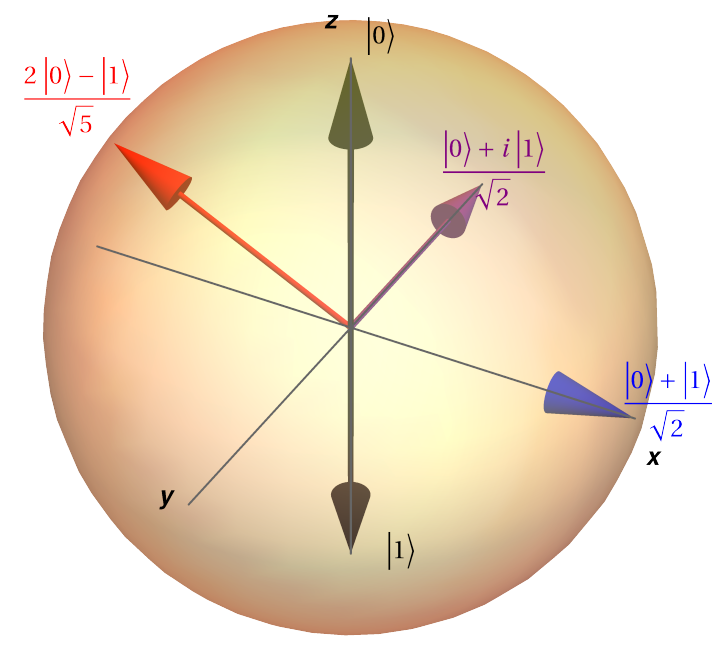
\includegraphics[width=5cm]{bloch.png}
\end{minipage}
$\stackrel{\E_{z}\otimes\1 \vspace{1cm}}{\longmapsto}$
\begin{minipage}{0.4\textwidth}
\centering
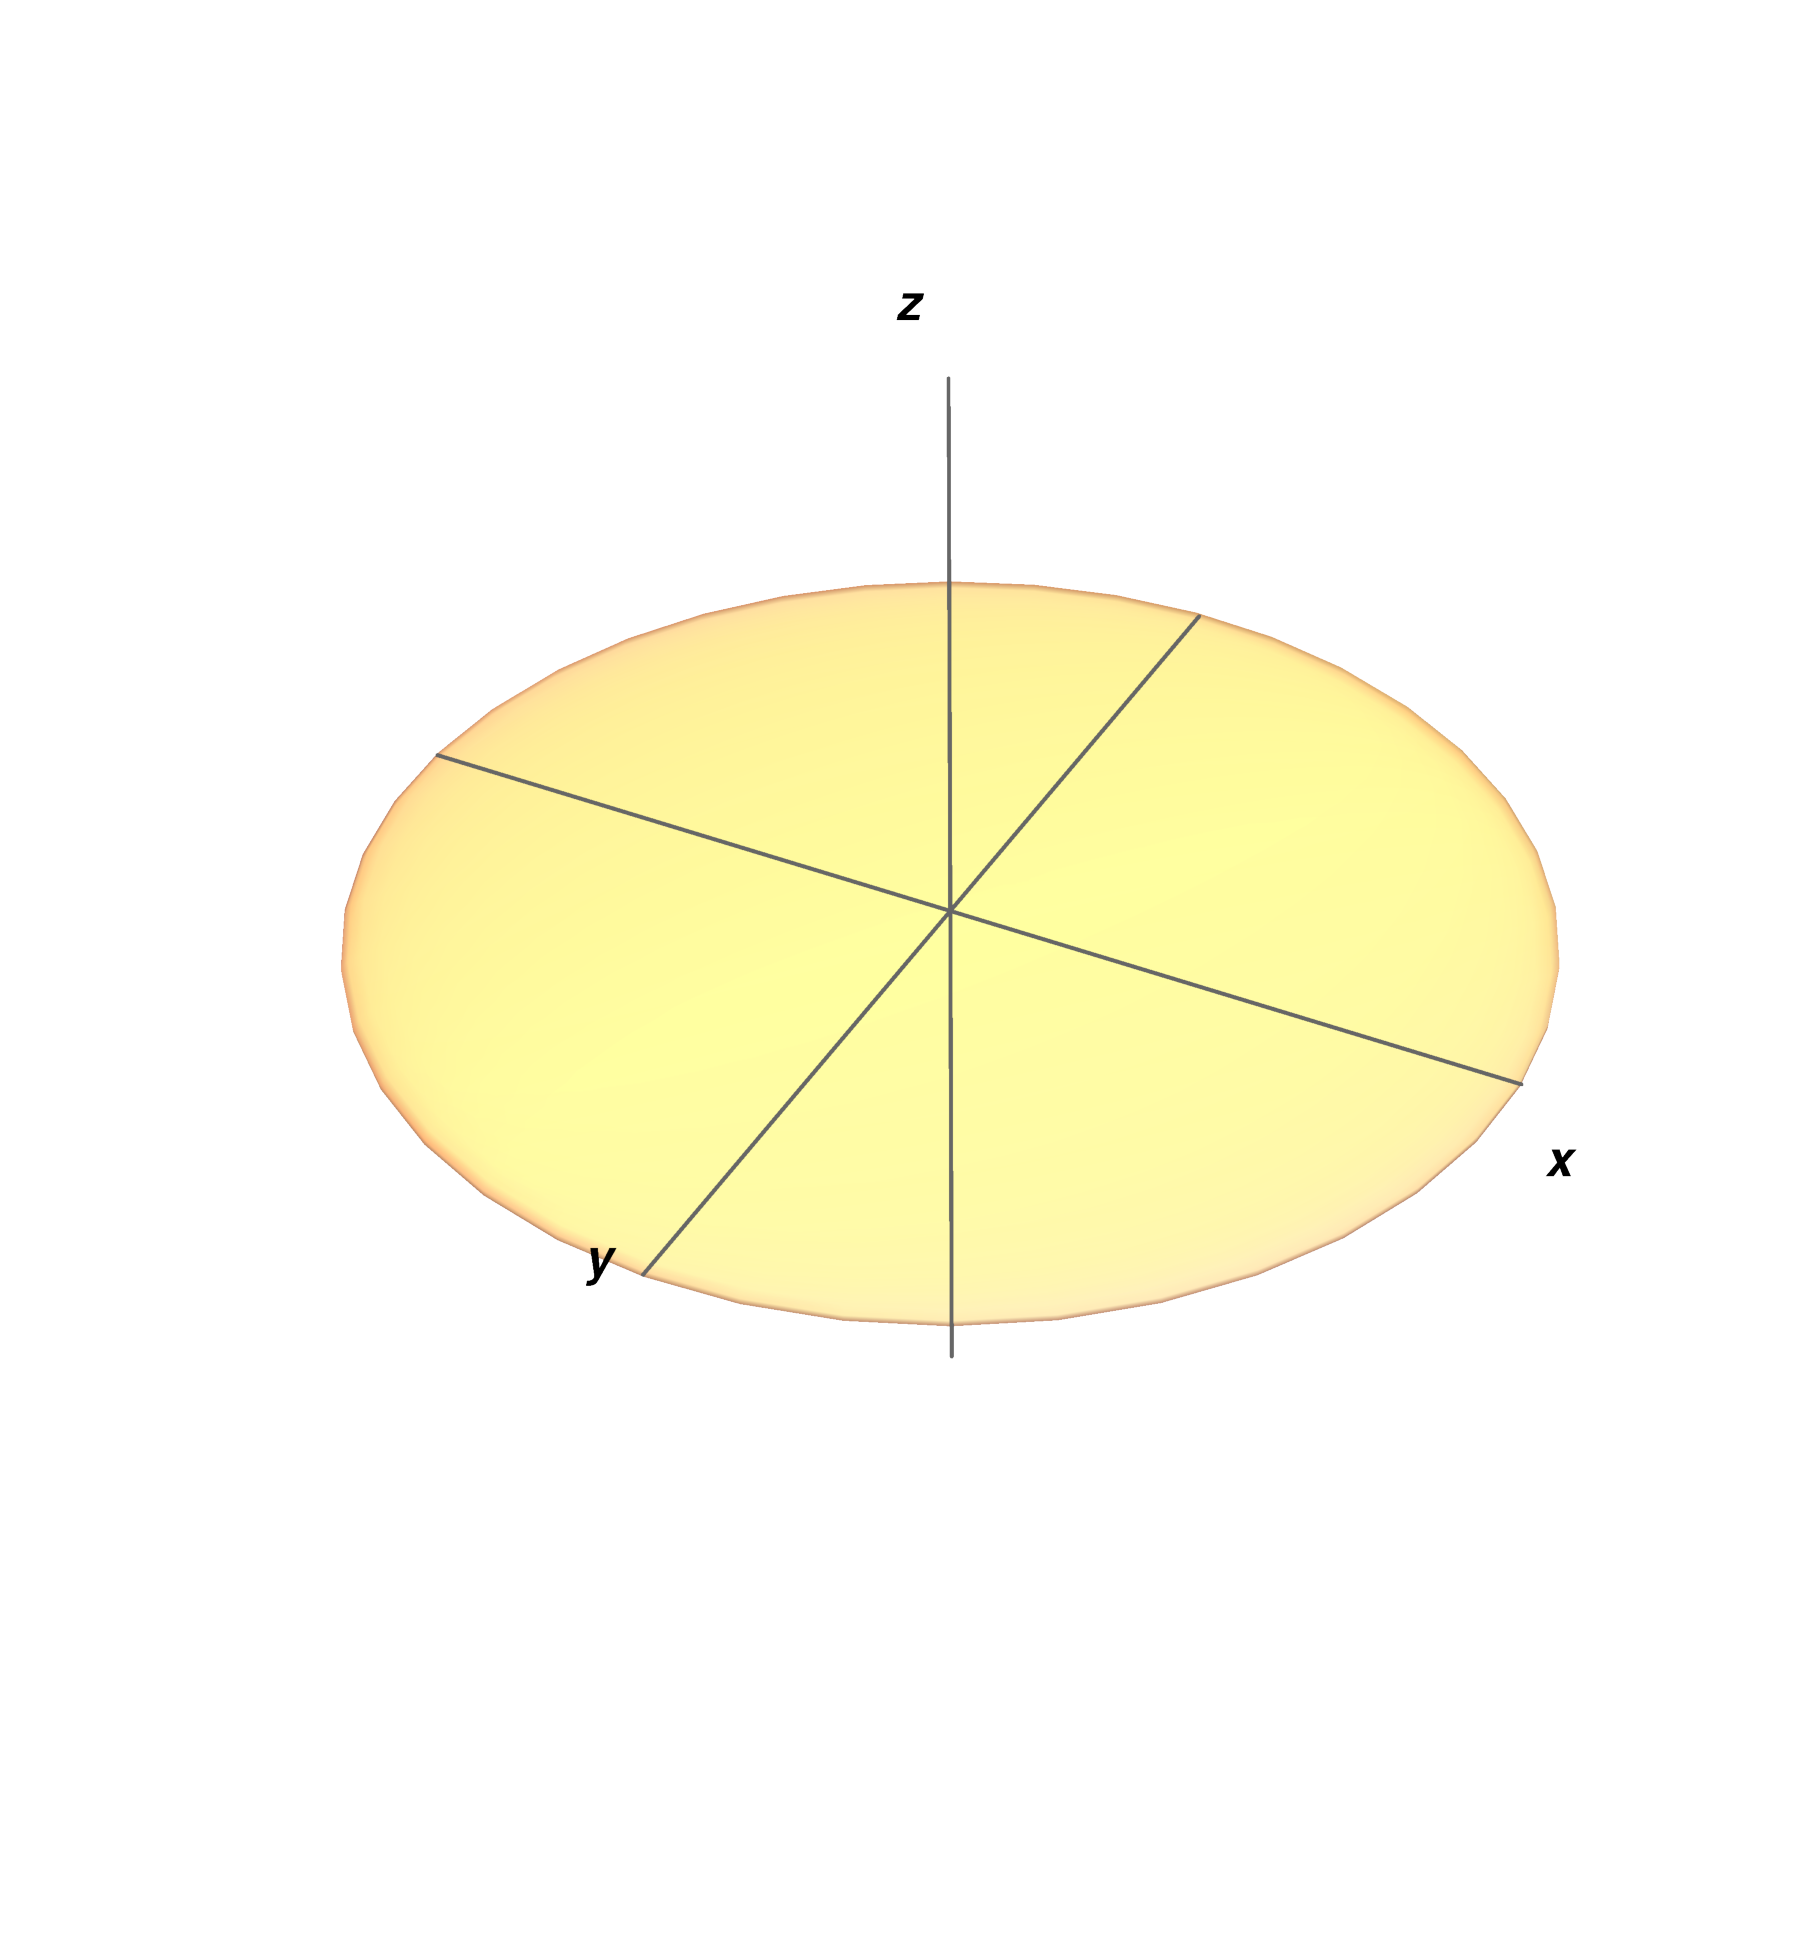
\includegraphics[width=6cm]{DiskXY}
\end{minipage}
\caption{Deformación de la esfera de Bloch a un disco sobre el plano $XY$. \ep}
\label{fig:qtm-op-motivation}
\end{figure} % }}}
Aunque podemos revisar explícitamente que las propiedades 
de traza unitaria y positividad de $\rho$ en \eqref{eq:rho-1qubit}
se preservan, también podemos argumentar geométricamente
que, dado que el disco final se contiene en la esfera de Bloch, 
las propiedades de la matriz densidad de 1 qubit se preservan.
Sin embargo, veremos que la acción de $\E_z\ot \1$ 
sobre el estado máximamente entrelazado de 2 qubits 
se transforma en una matriz no positiva.

Para 2 qubits, $\ket{\phi}=\qty(\ket{00}+\ket{11})/\sqrt{2}$ es el
estado máximamente entrelazado~\cite{bengtsson_zyczkowski_2017}.
Dado que conocemos cómo transforma $\E_z$ a la matriz densidad 
escrita en la base de matrices de Pauli será necesario calcular 
la representación de $\dyad{\phi}{\phi}$ escrita como en \eqref{eq:rho-2qubits}
para luego calcular $\E_z\ot \1(\dyad{\phi}{\phi})$.
Las componentes $r_{ij}$ se calculan usando el producto interno
de Hilbert-Schmidt $\Tr\qty(\pauli{i}{j}\dyad{\phi}{\phi})$~\cite{bengtsson_zyczkowski_2017}.
Así encontramos 
\begin{align}
\dyad{\phi}{\phi}=\frac{1}{4}\qty(
\pauli{0}{0}+\pauli{1}{1}-\pauli{2}{2}+\pauli{3}{3}).
\end{align}
Recordemos que $\E_z$ borra la componente $r_3$ de la
matriz densidad de 1 qubit en \eqref{eq:rho-1qubit}. 
Al calcular el superoperador $\E_z\ot  \1$, la representación matricial de 
un canal cuántico que veremos en la próxima sección, se encuentra
que $\E_z\otimes\1$ actuando sobre una matriz densidad de 2 qubits
escrita como en \eqref{eq:rho-2qubits} borra
las componentes de la forma $r_{3j}$. Por consiguiente
\begin{align}
\E_z\otimes\1 \qty(\dyad{\phi}{\phi})=\frac{1}{4}\qty(
\pauli{0}{0}+\pauli{1}{1}-\pauli{2}{2}),
\end{align}
que al calcular su representación matricial se tiene
\begin{align}
\E_z\otimes\1 \qty(\dyad{\phi}{\phi})=
\mqty( 
\frac{1}{4} & 0 & 0 & \frac{1}{2} \\
0 & \frac{1}{4} & 0 & 0 \\
0 & 0 & \frac{1}{4} & 0 \\
\frac{1}{2} & 0 & 0 & \frac{1}{4} \\
).
\end{align}

La matriz  $\E_z\otimes\1\qty(\dyad{\phi}{\phi})$ tiene un 
eigenvalor igual a $-1/4$ y, por lo tanto, no satisface la condición 
de positividad para ser una matriz densidad.  
En otras palabras, $\E_z\otimes\1\qty(\dyad{\phi}{\phi})$ 
no representa a un estado físico de 2 qubits y 
se dice entonces que $\E_z$ no es una operación completamente 
positiva porque existen estados en el espacio extendido de 2 qubits para 
el cual la extensión $\E_z\ot \1$ no preserva la positividad de esos estados. 
De esta manera acabamos de mostrar que la condición de completa
positividad surge de la posibilidad que un sistema tiene de encontrarse 
en un estado entrelazado con un \textit{ancilla}.

Ya que elaboramos la implicación física de la completa positividad 
vamos a establecer una definición precisa de esta condición con la
que debe de cumplir un canal cuántico.
Se dice que una operación $\E$ es CP si 
y sólo si, para cualquier extensión arbitraria de dimensión $K$ 
del espacio de Hilbert $(\hi_N \rightarrow \hi_N \otimes \hi_K)$ 
el operador $\E\otimes\1_K$ es positivo~\cite{bengtsson_zyczkowski_2017}. 
Con esta definición hemos terminado de revisar las dos condiciones que 
debe de satisfacer una operación lineal para ser un 
canal cuántico.

Un canal cuántico es un mapeo lineal que
\begin{enumerate} 
\item Preserva las características de la matriz densidad.
\item Es completamente positivo.
\end{enumerate}
En la literatura se suele utilizar el término operaciones 
completamente positivas que preservan la traza 
(CPTP por sus siglas en ingles, \textit{Completely Positive and
Trace-Preserving}) para referirse a los canales 
cuánticos~\cite{bengtsson_zyczkowski_2017}. 
En la siguiente y última sección de este capítulo estudiaremos 
algunas representaciones de canales cuánticos. 
% }}}
\section{Representaciones de los canales cuánticos} % {{{
\label{sec:qtm-channels-representation}
En esta sección estudiaremos dos representaciones distintas de 
los canales cuánticos: los superoperadores y la representación 
de suma de operadores de Kraus. Para cada una de ellas, vamos a revisar
cómo escribir las condiciones que hacen a una operación lineal un 
canal cuántico. La representación como superoperador 
será especialmente útil para investigar el problema
que vamos a plantear en el siguiente capítulo. No obstante, los 
operadores de Kraus siguen siendo una parte importante dentro 
de la teoría de los canales cuánticos y por eso dedicamos brevemente
la última parte de esta sección a estudiarlos.

Los canales cuánticos pueden entenderse como operadores 
que actúan sobre otros operadores. 
La matriz densidad actúa sobre 
el espacio de Hilbert y un canal cuántico actúa sobre las matrices de 
densidad, que forman parte del espacio de Hilbert-Schmidt. 
La diferencia es entonces que las matrices de densidad 
son operadores que actúan sobre el espacio de 
Hilbert y los canales cuánticos actúan sobre el espacio 
de Hilbert-Schmidt. Para hacer una diferencia en 
la naturaleza de los dos tipos de operadores, los canales cuánticos 
pueden recibir el nombre de superoperadores~\cite{preskill1998lecture}.

Vamos a revisar primero un cambio de notación que \textit{vectoriza} a la matriz densidad 
para después exponer cómo es la representación matricial de
un canal cuántico como un superoperador.
Consideremos una matriz densidad $\rho$ de dimensión $d\times d$.
Para vectorizar a $\rho$, los elementos de matriz $\rho_{ij}$ 
se deben acomodar en un vector columna $\vec{\rho}$, con componentes 
$\rho_k$, siguiendo la ecuación~\citep{bengtsson_zyczkowski_2017}
\begin{align}
\rho_k=\rho_{ij};\hspace{2cm} k=\qty(i-1)d+j,
\label{eq:matrix-to-vector}
\end{align}
donde $i,j=,1,\ldots,d$. Por ejemplo, la matriz densidad
\begin{align}
\rho=\mqty(\rho_{00}&\rho_{01}\\ \rho_{10}&\rho_{11})
\end{align}
que actúa sobre un espacio de Hilbert de dimensión 2 se vectoriza como 
\begin{align}
\vec{\rho}=\mqty(\rho_{00}\\ \rho_{01}\\ \rho_{10}\\ \rho_{11}).
\end{align}
En general, una matriz densidad $\rho$ que actúa 
sobre un espacio de Hilbert de dimensión $d$ es 
una matriz de dimensión $d\times d$. Si se vectoriza a $\rho$, la matriz 
de densidad se transforma en un vector $\vec{\rho}$ de $d^2$ 
componentes. Un canal cuántico $\E$ que actúa sobre $\rho$ se puede
representar entonces como una matriz de dimensión $d^2\times d^2$ 
que actúa sobre el vector $\vec{\rho}$. Esta representación matricial de 
$\E$ es la que se conoce como superoperador.

Antes de estudiar las condiciones que un superoperador $\E$
debe satisfacer para ser un canal cuántico es necesario que revisemos
dos herramientas algebraicas: (1) una notación de cuatro índices 
para los elementos de matriz de un operador, y (2) la transformación 
algebraica de \textit{reshuffle}. Primero, para introducir la nueva notación
consideremos a un superoperador $\E$ que actúa sobre un espacio de 
Hilbert-Schmidt de la forma $\hi\mathcal{S}_M\otimes\hi\mathcal{S}_N$. 
Sea $\ket{m}$ una base ortonormal de $\hi\mathcal{S}_M$, $\ket{\mu}$ 
una base ortonormal de $\hi\mathcal{S}_N$ y, por lo tanto, 
$\ket{m}\otimes\ket{\mu}$ una base ortonormal de 
$\hi\mathcal{S}_M\ot\hi\mathcal{S}_N$.
Nótese el uso de letras latinas para los índices del
primer subsistema y letras griegas para los índices del segundo. 
Utilizando cuatro índices, un elemento de matriz de $\E$ se calcula como
\begin{align}
\E_\ind{m\mu}{n\nu}=\matrixel{m\otimes \mu}{\E}{n\otimes \nu}.
\label{eq:4indices}
\end{align}
Por último, vamos a introducir la transformación algebraica de \textit{reshuffle}
de un superoperador $\E$ utilizando la nueva notación de cuatro índices 
en \eqref{eq:4indices}.
El \textit{reshuffle} $\E^R$ de un superoperador $\E$ se define 
como~\cite{bengtsson_zyczkowski_2017}
\begin{align}
\E^R_\ind{m\mu}{n\nu} = \E_\ind{mn}{\mu\nu}.
\label{eq:Reshuffle_4-indices}
\end{align}
El siguiente ejemplo ilustra cómo utilizar la notación de cuatro 
índices en \eqref{eq:4indices} y cómo hacer la transformación 
de \textit{reshuffle} en \eqref{eq:Reshuffle_4-indices} de un 
superoperador que actúa sobre un espacio de Hilbert-Schmidt de 
dimensión 4 de la forma $\mathcal{HS}_2\ot \mathcal{HS}_2$,
%\begin{align}
%\left(
%\begin{array}{cccc}
% \E_{11} & \E_{12} & \E_{13} & \E_{14} \\
% \E_{21} & \E_{22} & \E_{23} & \E_{24} \\
% \E_{31} & \E_{32} & \E_{33} & \E_{34} \\
% \E_{41} & \E_{42} & \E_{43} & \E_{44} \\
%\end{array}
%\right)^R
%=
%\left(
%\begin{array}{cccc}
% \E_{11} & \E_{12} & \E_{21} & \E_{22} \\
% \E_{13} & \E_{14} & \E_{23} & \E_{24} \\
% \E_{31} & \E_{32} & \E_{41} & \E_{42} \\
% \E_{33} & \E_{34} & \E_{43} & \E_{44} \\
%\end{array}
%\right).
%\end{align}
\begin{align}
\left(
\begin{array}{cccc}
 \E_{\ind{00}{00}} & \E_{\ind{00}{01}} & \E_{\ind{00}{10}} & \E_{\ind{00}{11}} \\
 \E_{\ind{01}{00}} & \E_{\ind{01}{01}} & \E_{\ind{01}{10}} & \E_{\ind{01}{11}} \\
 \E_{\ind{10}{00}} & \E_{\ind{10}{01}} & \E_{\ind{10}{10}} & \E_{\ind{10}{11}} \\
 \E_{\ind{11}{00}} & \E_{\ind{11}{01}} & \E_{\ind{11}{10}} & \E_{\ind{11}{11}} \\
\end{array}
\right)^R
=
\left(
\begin{array}{cccc}
 \E_{\ind{00}{00}} & \E_{\ind{00}{01}} & \E_{\ind{01}{00}} & \E_{\ind{01}{01}} \\
 \E_{\ind{00}{10}} & \E_{\ind{00}{11}} & \E_{\ind{01}{10}} & \E_{\ind{01}{11}} \\
 \E_{\ind{10}{00}} & \E_{\ind{10}{01}} & \E_{\ind{11}{00}} & \E_{\ind{11}{01}} \\
 \E_{\ind{10}{10}} & \E_{\ind{10}{11}} & \E_{\ind{11}{10}} & \E_{\ind{11}{11}} \\
\end{array}
\right).
\end{align}
La transformación de \textit{reshuffle} nos será útil específicamente 
para entender la condición de completa positividad que un superoperador $\E$
de cumplir para ser un canal cuántico.

Ahora que ya contamos con las herramientas algebraicas necesarias
estamos listos para enunciar las condiciones que debe cumplir un 
superoperador $\E$ para ser un canal cuántico. 
%Un superoperador 
%$\E$ es una matriz que actúa sobre una matriz densidad vectorizada
%$\vec{\rho}$\cpnote{Quitaría esta frase. Para ser superoperador, actua sobre cualquier
%operador. Ya lo dijiste arriba y creo que acá no mas estas metiendo ruido}.
Recordemos de la sección anterior que un canal cuántico 
es una operación lineal que actúa sobre una matriz densidad 
como en \eqref{eq:E(rho)}, donde $\rho'$
es una matriz densidad y $\E$ es una operación completamente positiva.
La condición de positividad con la que debe cumplir la matriz densidad 
implica que además es una matriz Hermítica. 
Por lo tanto, que un canal cuántico preserve la Hermiticidad, traza unitaria 
y positividad de la matriz densidad impone tres condiciones 
sobre el superoperador $\E$~\cite{bengtsson_zyczkowski_2017}:
% \janote{Sobre la hermiticidad de $\rho$: es una propiedad que se puede 
% deducir de la positividad: si $\rho$ es positiva tiene descomposición 
% espectral $\sum_i\lambda_i\dyad{\psi_i}{\psi_i}$,
% entonces se sigue que $\rho=\rho^{\dagger}$. Por eso, arreglé este
% párrafo que acabas de terminar de leer para introducir la Hermiticidad
% como una propiedad que se deduce de las características de la 
% matriz densidad que establece el teorema \ref{teo:density-matrix}.}
% \cpnote{No has definido rho prima (al menos no cerca), para que tngan sntido
% estas definiciones, tienes que decir de neuvo que rho prima es E sobre rho}
% \janote{Listo. Leete de nuevo este párrafo. Borré el enunciado que 
% comentaste que hacía ruido.}
\begin{align}
\txt{(i)}&& \rho'&=\qty(\rho')^{\dagger}&\Leftrightarrow
    && \E_\ind{m\mu}{n\nu}=\E_\ind{\mu m}{\nu n}^*,&&
    \label{eq:H-condition}\\
\txt{(ii)}&&\Tr(\rho')&=1
    &\Leftrightarrow&&  \sum_{m}\E_\ind{mm}{n\nu}=\delta_{n\nu},&
    \label{eq:Tr-condition}\\     
\txt{(iii)}&&\matrixel{\psi}{\rho'}{\psi}&\geq0,\ \forall \ket{\psi} \in \hi
    &\Leftrightarrow&&  \sum_{n\nu}\E_{\ind{m\mu}{n\nu}}\rho_{n\nu}\geq0,& 
    & \rho>0.
    \label{eq:positivity-condition}
\end{align}
De esta manera, solo nos hace falta revisar la condición que debe cumplir
un superoperador $\E$ para ser una operación completamente positiva.
% \cpnote{no entiendo esta frase en este contexto. estamos evaluando algo? Ya
% evaluamos algo? Además creo que aca conviene separar parrafo pues pasas
% de algo general a lo particular. Como que siento qeu aca el flujo esta chistoson. 
% Dale una mirada a esto y le sigo luego} \janote{Listo. Reformulé lo que 
% quería decir con `evaluar'}
Para eso, se introduce a la matriz de Choi $D_{\E}$ de $\E$,
que se define como~\cite{bengtsson_zyczkowski_2017}
\begin{align}\label{eq:ChoiMatrix-via-reshuffle}
D_{\E}=\E^{R},
\end{align}
con $\E^R$ la transformación de \textit{reshuffle} definida en 
\eqref{eq:Reshuffle_4-indices}. El siguiente teorema establece 
cuándo $\E$ es una operación completamente positiva:
\begin{thm}{Teorema de Choi.}\label{thm:choi-CP}
Un superoperador lineal $\E$ es completamente positivo si y sólo si 
su matriz de Choi asociada $D_{\E}$ es positiva semidefinida.
\end{thm}
\begin{proof}
Vamos a presentar la demostración expuesta por Bengtsson
en~\cite[p. 281]{bengtsson_zyczkowski_2017}.
La matriz de Choi $D_{\E}$ de un 
canal cuántico $\E$ es una matriz hermítica que 
actúa sobre el espacio de Hilbert-Schmidt $\mathcal{H}_{N^2}$
(espacio de las matrices de dimensión $N^2\times N^2$). 
Por el teorema de descomposición espectral, 
la matriz $D_{\E}$ se puede escribir~\cite{nielsen_chuang_2011}
\begin{align}\label{eq:choiThmProof_braketChoi}
D_{\E}&=\sum_{i}\lambda_i\dyad{\chi_i}{\chi_i},
\end{align}
con $\lambda_i$ sus eigenvalores. Dado que la matriz de Choi es una 
matriz Hermítica, $\lambda_i\in\mathbb{R}$. En la notación 
de cuatro índices introducida en \eqref{eq:4indices},
\eqref{eq:choiThmProof_braketChoi} se escribe
\begin{align}
D_{\ind{mn}{\mu\nu}}&=\sum_i\lambda_i
\chi^i_{mn}\qty(\chi_{\mu\nu}^i)^*.
\end{align}
Consideremos la acción de $\E\ot \1_N$ sobre un 
estado puro $z_{nn'}z^*_{\nu\nu'}$ de $\mathcal{H}_{N^2}$,
\begin{align}
\rho'_{mm'\mu\mu'}&=
\sum_{n,n',\nu,\nu'}
\E_{\ind{m\mu}{n\nu}}\delta_{\ind{m'\mu'}{n'	\nu'}}z_{nn'}z^*_{\nu\nu'}
=
\sum_{n,\nu}
\E_{\ind{m\mu}{n\nu}}z_{nm'}z^*_{\nu\mu'},
\end{align}
donde $\delta_{\ind{m'\mu'}{n'	\nu'}}=\delta_{m'n'}\delta_{\mu'\nu'}$,
\begin{align}
\sum_{n,\nu}\E_{\ind{m\mu}{n\nu}}z_{nm'}z^*_{\nu\mu'}&=
\sum_{n,\nu}D_{\ind{mn}{\mu\nu}}z_{nm'}z^*_{\nu\mu'}\nonumber\\
\rho'_{mm'\mu\mu'}&=
\sum_{n,\nu,i}\lambda_{i}
\chi^i_{mn}z_{nm'}\qty(\chi_{\mu\nu}^iz_{\nu\mu'})^*.
\label{eq:rho'_ChoiThmProof}
\end{align}
%%%%%%%%%%
% \here
% Nótese que utilizamos la definición de la matriz de Choi via 
% el \textit{reshuffle} del superoperador $\E$, 
% $\E_{\ind{m\mu}{n\nu}}=\E^R_{\ind{mn}{\mu\nu}}
% =D_{\ind{mn}{\mu\nu}}$.
% Finalmente, para determinar \cpnote{me parece que acá va ``determinar''
% (moidificando un poco la frase que sigue) o ``si requerimos\ldots'' algo asi.
% No lo cambio porque quiero resaltar que creo que abusas de la palabra
% ``evaluar''}\janote{Por favor revisa de nuevo esta demostración completa.
% Con tus comentarios me di cuenta que tenía errores, 
% hice cambios para que todo el flujo de ideas se entendiera mejor.
% Si está bien porga quita lo que se encuentra entre los \texttt{$\setminus$here}} si $\rho'$ es una matriz positiva 
% revisamos que el valor esperado de ella con un vector arbitrario~$y_{mm'}$
% \cpnote{Uno calcula los elementos de matriz con respecto a una base. Quizá
% lo que quieres hacer es calcular un valor esperado.}
% es no negativo,
% \here
%%%%%%%%%%
Por último, utilizamos el hecho de que $\rho'$ debe ser una matriz 
de densidad y, por ende, una matriz positiva semidefinida,
\begin{align}
\sum_{m,m',\mu,\mu'}
y_{mm'}\rho'_{mm'\mu\mu'}y^*_{\mu\mu'}
\geq0,
\end{align}
con $y_{mm'}$ un vector arbitrario de $\mathcal{H}_{N^2}$.
Utilizamos \eqref{eq:rho'_ChoiThmProof} para sustituir $\rho'$,
\begin{align}
\sum_{m,m',n,n'}\lambda_i\abs{y_{mn'}\chi^i_{mn}z_{nm'}}^2\geq0.
\end{align}
Para que esto sea cierto para cualesquiera vectores $z_{mm'}$ y  
´$y_{mm'}$, se debe de cumplir que $\lambda_i\geq0$. Recordemos
que $\lambda_i$ son los eigenvalores de $D_{\E}$.
En conclusión, para que $\rho'$ sea una matriz positiva, la matriz de Choi 
$D_{\E}$ también debe ser una matriz positiva. 
%%%%%%%%%%
% \here
% Por consiguiente, la matriz 
% de Choi $D_{\E}$ debe ser positiva semidefinida para que $\rho'$ 
% también lo sea. \cpnote{No lo veo. Explicamelo, o si puedes 
% poner una ecuación matricial, estaría padre.}\newline \noindent
% \here
%%%%%%%%%%
\end{proof}
En resumen, un superoperador $\E$ es un canal cuántico si 
cumple con las tres condiciones establecidas en las ecuaciones 
\eqref{eq:H-condition}, \eqref{eq:Tr-condition}
y \eqref{eq:positivity-condition}, además de lo que establece 
el teorema \ref{thm:choi-CP}, que su matriz de Choi sea 
positiva semidefinida. 

Vamos a terminar este primer capítulo presentando 
brevemente la representación en operadores de Kraus 
de un canal cuántico. Los operadores de Kraus fueron 
introducidos por Karl Kraus en 1971 como una consecuencia
deducida por él del teorema de Stinespring para las operaciones 
completamente positivas~\cite{bengtsson_zyczkowski_2017}. 
Aunque la representación en operadores de Kraus y los
superoperadores puedan parecer fundamentalmente distintos, 
ambas representaciones guardan conexión mediante 
la matriz de Choi de un canal cuántico.

A diferencia de un superoperador, los operadores de Kraus representan
a un canal cuántico con operadores que actúan sobre el espacio 
de Hilbert, igual que las matrices de densidad. En la representación 
de Kraus, un canal cuántico $\E$ actúa sobre la matriz 
de densidad como
\begin{align}\label{eq:KrausRepresentation}
\E\qty(\rho)=\sum_k E_k\rho E_k^{\dagger},
\end{align}
para algún conjunto de operadores $\{E_k\}$ que satisfacen la 
condición~\cite{nielsen_chuang_2011}
\begin{align}
\sum _kE_k^{\dagger}E_k\leq\1,
\end{align} 
donde los operadores $E_k$ reciben el nombre de operadores de Kraus.
La libertad de la representación de Kraus permite que 
varios conjuntos distintos de operadores $\{E_k\}$ sean la representación
de un mismo canal cuántico. Por ello, es de interés
determinar un conjunto canónico de operadores de Kraus.

El conjunto canónico se puede determinar para todas las operaciones 
completamente positivas a partir de su matriz de Choi. Un mapeo 
completamente positivo $\E:\mathcal{M}_d\footnote{Espacio de 
las matrices de dimensión $d\times d$.}\to\mathcal{M}_d$ 
se puede escribir como~\citep{bengtsson_zyczkowski_2017}
\begin{align}
\E(\rho) = 
\sum_{k=1}^{r\leq d^2}\lambda_k\chi_k\rho\chi_k^{\dagger}
%= \sum_{i=1}^rE_k\rho E_k^{\dagger},
\label{eq:Kraus-canonical}
\end{align}
con $\lambda_k$ y $\chi_k$ los eigenvalores y eigenvectores 
normalizados de la matriz de Choi $D_{\E}$, así como $r$ el rango 
de $D_{\E}$. 
Estrictamente hablando, $\chi_k$ son los eigenvectores reordenados 
como matrices según \eqref{eq:matrix-to-vector}.
Comparando las ecuaciones \eqref{eq:KrausRepresentation} y
\eqref{eq:Kraus-canonical}, los operadores de Kraus canónicos 
se definen como $E_k=\sqrt{\lambda_k}\chi_k$ y deben satisfacer
la condición
\begin{align}
  \Tr\qty(E_i^{\dagger}E_j)=d_i\delta_{ij}.
  \label{eq:Tr-Kraus-canonical}
\end{align}
Por último, ya que $\E$ es una operación que preserva la traza de 
la matriz densidad, debe imponerse la ecuación de completitud 
sobre los operadores canónicos de Kraus,
\begin{align}
  \sum_kE_k^{\dagger}E_k=\1.
%  \hspace{0.5cm}
%  \Rightarrow\hspace{0.5cm}
%  \sum_{k=1}^r\lambda_k=N .
  \label{eq:completeness-Kraus-canonical}
\end{align}
% \cpnote{no entiendo ni la flecha de la ecuación anterior ni el hecho de uqe sumen 
% a $N$} \janote{Era un ``por consiguiente''. Estuve pensando un rato 
% cómo explicar que era 'obvio' que suman N, pero no encontré cómo 
% así que lo comenté.
% Yo creo que no quita nada si sólo omito esa parte. Qué dices? }
En pocas palabras, un canal cuántico en la representación canónica de 
Kraus se escribe en la forma de \eqref{eq:Kraus-canonical}
siempre que los operadores canónicos de Kraus cumplan con 
la condiciones en \eqref{eq:Tr-Kraus-canonical} y 
\eqref{eq:completeness-Kraus-canonical}. 

Resumiendo, introdujimos brevemente 
% \cpnote{Creo que es un poco mucho decir que 
% revisamos esos formalismos. Mas bine se introdujeron brevemente o algo así.}
% \janote{Jajaja sí, estoy de acuerdo. Apenas y escupí la representación de Kraus.} 
el formalismo de la matriz densidad
y la teoría de los canales cuánticos. Por un lado, la matriz densidad es una 
matriz positiva de traza unitaria que sirve de herramienta para 
representar a los estados cuánticos. 
Por otro lado, la teoría de los canales cuánticos es un marco teórico 
para describir la evolución discreta de los sistemas cuánticos abiertos. 
Un canal cuántico es una operación completamente positiva que 
preserva la traza de la matriz densidad y se puede representar 
como superoperador o en la representación de 
suma de operadores de Kraus. La matriz densidad y los canales 
cuánticos son el marco teórico dentro del cual estudiaremos, en 
el resto de este trabajo, un tipo de operaciones muy particulares 
que actúan sobre sistemas de qubits, operaciones que hemos bautizado 
con el nombre de operaciones que borran las componentes de Pauli.

% \cpnote{Bien, va quedando bonita la tesis.}
% }}}

